\documentclass[a4,10pt]{article}

\usepackage[utf8]{inputenc}
\usepackage[english,spanish]{babel}
\usepackage{verbatim}
\usepackage{graphicx}
\usepackage{amsmath}
\usepackage{hyperref}

\begin{document}

\title{Aplicaciones de Geometría Proyectiva}
\author{Gustavo Quesada Menchón}
\date{}
\maketitle
\newpage

\tableofcontents
\newpage

\section{Introducción}

Este documento va ha tratar sobre geometría proyectiva y sus aplicaciones, de cómo con sus operaciones básicas nos facilita la tarea en aplicaciones como el tratamiento de imágenes, reconocimiento facial, visión estereoscópica, etc. Para abordar el tema, se va dividir en varias partes. Una pequeña introducción con un poco de historia, definiciones y conceptos básicos sobre geometría proyectiva. Una segunda parte donde se explican un poco las principales operaciones/transformaciones que nos pueden ser útiles. Una tercera parte donde se profundiza algo más en técnicas aplicadas en el tratamiento de imágenes 3D que se ha utilizado en algunos proyectos, y una parte final, con un pequeño resumen y conclusiones sobre el tema.


%%%%%%%%%%%%%%%%%%%%%%%%%%%%%%%%%%%%%%%%%%%%%%%%%%%%%%%%%%%%%%%%%%%%%%
\section {Definición y conceptos básicos}

Para comenzar explicando qué es la geometría proyectiva, veamos un poco de historia:

\emph{“
Gérard Desargues es el iniciador de la geometría proyectiva, pues fundamentó matemáticamente los métodos de la perspectiva que habían desarrollado los artistas del Renacimiento, y aunque su trabajo fue publicado en 1639, pasó desapercibido durante dos siglos (excepto dos teoremas), ensombrecido por la influyente obra de Descartes.\\
En el siglo XIX, la geometría proyectiva y la geometría hiperbólica, se establecieron dentro de las matemáticas, pero lo que acabó de enraizarlas, posiblemente, fue hallar un modelo analítico. Dentro del contexto de la geometría euclidiana-cartesiana se puede construir la geometría proyectiva, y si se acepta la primera, hay que admitir la segunda. Este proceso finalizó definitivamente a principios del siglo XX, pues Einstein, apoyándose en los exhaustivos desarrollos geométricos de los matemáticos del siglo XIX, consiguió demostrar que, a gran escala, el universo se puede interpretar mejor con estas nuevas geometrías que con el rígido espacio euclidiano.”}\\%poner por aqui una referencia a wikipedia, o al final
\\
Se podría decir que este interés por desarrollar la geometría proyectiva se debe al cambio en la temática de la pintura, ya que surge de la preocupación del artista de representar el mundo tridimensional en su lienzo bidimensional. En el periodo medieval las pinturas eran de carácter principalmente religioso y los pintores representaban a los personajes y objetos de una forma sumamente estilizada, generalmente sobre fondo dorado, para subrayar que el cuadro no tenía conexión con el mundo real. En el Renacimiento con la llegada del humanismo y el antropocentrismo la pintura se centra en la representación del mundo real.

Una vez establecidos los orígenes, podemos dar alguna definición breve:\\
\emph{
Se llama geometría proyectiva a la rama de la matemática que estudia las propiedades de incidencia de las figuras geométricas, pero abstrayéndose totalmente del concepto de medida.}\\

La geometría proyectiva puede entenderse, informalmente, como la geometría que se obtiene cuando nos colocamos en un punto, mirando desde ese punto. Esto es, cualquier línea que incide en nuestro ojo nos parece ser sólo un punto, en el Plano proyectivo, ya que el ojo no puede ver los puntos que hay detrás.
De esta forma, la geometría proyectiva también equivale a la proyección sobre un plano de un subconjunto del espacio en la geometría euclidiana tridimensional. Las rectas que salen del ojo del observador se proyectan sobre puntos. Los planos definidos por cada par de ellas se proyectan sobre rectas.

La geometría proyectiva también es aquella que trata las propiedades que se conservan bajo proyecciones. Tiene aplicaciones en visión artificial, funcionamiento de cámaras, reconstrucción de imágenes bidimensionales en tres dimensiones, etc. En resumen es la geometría asociada al modo en que el ojo humano percibe el mundo.

\section{Propiedades, operaciones y transformaciones más usadas}

Vamos a tratar en este apartado las transformaciones relacionadas con el tratamiento de imágenes en 3D. Para ello también será necesario explicar alguna de las ventajas que nos ofrece la geometría proyectiva.\\
\begin{enumerate}

\item \textbf{Transformaciones proyectivas 3D}\\
En las transformaciones geométricas de un sistema cartesiano 3D, un punto en el espacio se define por las coordenadas (X, Y, Z) y un pixel en la imagen por el par de coordenadas (x, y).
A continuación se presentan las transformaciones geométricas 3D fundamentales para el tratamiento de imágenes en tres dimensiones, la rotación y traslación. 
En la figura (Fig. \ref{fig:fig1})se presenta un sistema de coordenadas 3D (X, Y, Z) que ha sufrido una transformación de translación y rotación. El sistema nuevo generado como resultado de dicha transformación es el definido por (X’, Y ’, Z’). La ecuación que relaciona ambos sistemas de coordenadas es la siguiente: 

\begin{equation}
\begin{pmatrix}
X'\\
Y'\\
Z'
\end{pmatrix}
= R
\begin{pmatrix}
X\\
Y\\
Z
\end{pmatrix}
+ t
\end{equation}

donde t es un vector 3 x 1 que identifica la translación y R es una matriz 3 x 3 que representa la rotación del sistema de coordenadas.

\underline{Rotación}\\
En el escenario 3D, la matriz R se define de manera particular para cada uno de los ejes. De esta manera, una transformación de rotación se descompone en tres subrotaciones:\\
\begin{equation}
R_Z =
\begin{bmatrix}
\cos(\omega Z) & \sin(\omega Z) & 0\\
-\sin(\omega Z) & \cos(\omega Z) & 0\\
0 & 0 & 1\\
\end{bmatrix}
\end{equation}
\begin{equation}
R_Y =
\begin{bmatrix}
\cos(\omega Y) & \sin(\omega Y) & 0\\
0 & 1 & 0\\
\sin(\omega Y) & 0 & \cos(\omega Y)\\
\end{bmatrix}
\end{equation}
\begin{equation}
R_X =
\begin{bmatrix}
1 & 0 & 0\\
0 & \cos(\omega X) & \sin(\omega X)\\
0 & -\sin(\omega X) & \cos(\omega X)\\

\end{bmatrix}
\end{equation}

Como se trata de aplicaciones lineales, las tres rotaciones pueden combinarse formando una única expresión de rotación global. Matemáticamente se expresa como la multiplicación de todas ellas.\\
\begin{equation}
R (\omega X , \omega Y , \omega Z ) = R_X (\omega X ) R_Y (\omega Y ) R_Z (\omega Z )
\end{equation}

\underline{Traslación}\\
La transformación de translación se modela a partir de un vector. De esta manera:\\
\begin{equation}
\begin{pmatrix}
X'\\
Y'\\
Z'
\end{pmatrix}
=
\begin{pmatrix}
X\\
Y\\
Z
\end{pmatrix}
+ t
\end{equation}

donde t es un vector de dimensiones 3 x 1.\\
\begin{figure}
\begin{center}
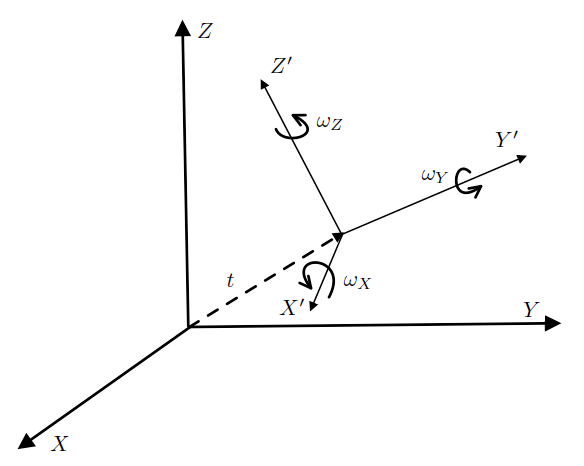
\includegraphics[width=0.5\linewidth]{images/figura1}
\end{center}
\caption{Coodenadas 3D, traslación y rotación}
\label{fig:figura1}
\end{figure}
Las dos transformaciones númeradas aquí se ven beneficiadas de la cualidad de la geometría proyectiva de operar con coordenadas homogéneas, lo cuál facilitará la resolución de las ecuaciones como se comenta en el siguiente punto.

\item \textbf{Coordenadas Homogéneas}\\
Las coordenadas homogéneas permiten combinar las transformaciones de rotación y translación en una única matriz. De esta manera, se consiguen expresiones compactas que posibilitan realizar los cálculos proyectivos de manera más eficiente.\\ 
En matemáticas, y de manera más concreta en el ámbito de la geometría proyectiva, las coordenadas homogéneas representan un instrumento fundamental para describir un punto en el espacio proyectivo. Dado el punto M de coordenadas cartesianas (X, Y, Z), se definen sus coordenadas homogéneas como (kX, kY, kZ, k), donde k es una constante distinta de cero. Para el caso particular de k = 0, dicho vector representa una dirección. La transformación entre ambos tipos de coordenadas es trivial y consiste en dividir los tres primeros términos de coordenadas homogéneas por el último.


\end{enumerate}
%%%%%%%%%%%%%%%%%%%%%%%%%%%%%%%%%%%%%%%%%%%%%%%%%%%%%%%%%%%%%%%%%%%%%%

\section{Aplicaciones en la realidad}



%%%%%%%%%%%%%%%%%%%%%%%%%%%%%%%%%%%%%%%%%%%%%%%%%%%%%%%%%%%%%%%%%%%%%

\section{Conclusión}


\bibliographystyle{plain}
\bibliography{refs}

\end{document}
